\chapter{Laws of Nature, Four-Vectors, and Tensors}

This lecture is really about the form that laws of nature must take. Following Leonard Susskind's order of attack, and curated here by LazyingArt LLC, we begin with a deliberately bad law, repair it by demanding invariance under rotations and then under Lorentz transformations, and only after that introduce the notation of four-vectors, scalars, and tensors. Throughout most of the chapter we set \(c=1\); when useful, we briefly restore \(c\) to make the nonrelativistic limit transparent.

\section{Symmetry As The First Test Of A Law}

Suppose we invent a possible law of nature: two particles interact whenever their \(x\)-coordinates become equal. There is no logical contradiction in such a rule. One can perfectly well write
\begin{equation}
x_1-x_2=0.
\end{equation}
If that equation holds, the particles suddenly change direction, or bounce, or do whatever our imagined law tells them to do.

The point of the example is not that such a law is mathematically impossible. The point is that it does not have the right form. It singles out one component of position and treats it as special. The law has been written in a way that depends on the orientation of our axes.

\subsection{Question \& Answer}

\paragraph{What symmetry is actually being violated?}

A natural first guess is homogeneity of space. But that is not the right diagnosis. The rule \(x_1-x_2=0\) does not pick out any preferred value of \(x\); it survives a translation of the origin. What it violates is isotropy of space. If we rotate the axes by \(90^\circ\), the same physical rule would now have to say that particles collide when their \(y\)-coordinates are equal. The form of the law changes under a rotation, and that is precisely what ought not to happen.

This is the first lesson of the lecture. Laws of nature are not merely statements that happen to be true in one chosen coordinate system. They should survive a change of coordinates without changing their essential form.

\section{From Spatial Coincidence To Spacetime Coincidence}

The repair is immediate. Instead of demanding equality of one component, we demand equality of position itself. In two or three dimensions, the particles interact only when they arrive at the same point in space. If \(\vec r_1\) and \(\vec r_2\) are their position vectors, the collision rule becomes
\begin{equation}
\vec r_1=\vec r_2,
\qquad\text{or equivalently}\qquad
\vec r_1-\vec r_2=\vec 0.
\end{equation}
Now the statement is rotationally invariant. A vector that is zero in one coordinate system is zero in every rotated coordinate system. Likewise, if two vectors are equal in one frame, they are equal in every rotated frame. This is why vector equations are the natural language for rotationally invariant physics.

At this point Susskind deliberately postpones time, and then brings it back in. One could try a Newtonian-looking rule that says particles collide only when their times are equal. That is a perfectly sensible statement in pre-relativistic physics, but it is not Lorentz invariant. Simultaneity is frame-dependent. A condition on the time component alone cannot be the final form of a relativistic law.

The relativistic repair is exactly parallel to the spatial one. Two collision events must coincide as a whole spacetime event. If \(X^\mu\) denotes the spacetime location of an event, then a simple collision law takes the form
\begin{equation}
X_1^\mu=X_2^\mu,
\qquad\text{or}\qquad
X_1^\mu-X_2^\mu=0.
\end{equation}
The important point is not just that one can write this equation. The important point is that one is now speaking about the entire four-vector, not about one preferred component.

\section{Four-Vectors And Matrix Form Of Transformations}

A four-vector is an object whose four components transform exactly as the coordinates of spacetime do. In the lecture the ordering is \((1,2,3,0)\), with the time component labeled by \(0\). Thus we may write
\[
X^\mu=(x^1,x^2,x^3,x^0)=(x,y,z,t).
\]

For a boost in the \(x\)-direction, the lecture uses the standard relativistic formulas, written with \(c=1\):
\begin{align}
x'&=\gamma(x-vt),&
y'&=y,&
z'&=z,&
t'&=\gamma(t-vx),
\end{align}
where
\begin{equation}
\gamma=\frac{1}{\sqrt{1-v^2}}.
\end{equation}
The transcript is noisy around some of the board writing, but the standard boost formulas are clearly what is intended.

A rotation about the \(z\)-axis has a different content but the same structural feature: the equations are linear, and only certain components mix. In cleaned form,
\begin{equation}
\begin{pmatrix}
x'\\
y'\\
z'\\
t'
\end{pmatrix}
=
\begin{pmatrix}
\cos\theta & \sin\theta & 0 & 0\\
-\sin\theta & \cos\theta & 0 & 0\\
0 & 0 & 1 & 0\\
0 & 0 & 0 & 1
\end{pmatrix}
\begin{pmatrix}
x\\
y\\
z\\
t
\end{pmatrix}.
\end{equation}
Here again we are normalizing the lecture to the standard \(z\)-axis rotation matrix, since the transcript around the explicit coefficients is partially corrupted.

What matters most for the rest of the lecture is that both boosts and rotations are linear operations. That is exactly what the board is emphasizing when it shifts from component-by-component formulas to indexed and matrix notation.

\begin{figure}
\centering

\includegraphics[width=0.68\textwidth]{lecture_06_figure_03.png}
\caption{Indexed Lorentz transformation and the beginning of its column-vector form on the board.}
\end{figure}

The cleaned indexed form is
\begin{equation}
X'^{\mu}=L^{\mu}{}_{\nu}X^{\nu}.
\end{equation}
This means that the primed component with index \(\mu\) is obtained by summing over the repeated index \(\nu\). The repeated one-up/one-down index is nothing mysterious; it is simply the matrix multiplication rule written compactly.

The corresponding column-vector form is
\begin{equation}
\begin{pmatrix}
x'\\
y'\\
z'\\
t'
\end{pmatrix}
=
L
\begin{pmatrix}
x\\
y\\
z\\
t
\end{pmatrix}.
\end{equation}
From here the definition of a four-vector becomes operational: any object \(A^\mu\) is a four-vector if it transforms in the same way,
\begin{equation}
A'^{\mu}=L^{\mu}{}_{\nu}A^{\nu}.
\end{equation}
Once we write laws in terms of such whole objects, their form can survive the move from one inertial frame to another.

\section{Scalars, Lowered Indices, And Invariants}

Before going further with vectors, the lecture slows down and backs up to something simpler: scalars. A scalar is a quantity that does not change under the transformation in question. Temperature at a point is a scalar under spatial rotations. The distance between two points in space is also a scalar. If two quantities are both scalars, then the statement that they are equal is automatically rotationally invariant.

Vectors are different. Their individual components do change. That is why we must learn to form combinations of components that do not change.

Let \(A^\mu\) be a general four-vector. The lecture distinguishes its contravariant components \(A^\mu\) from its covariant components \(A_\mu\). The latter are obtained by multiplying by the metric:
\begin{equation}
A_{\mu}=\eta_{\mu\nu}A^{\nu},
\qquad
\eta_{\mu\nu}=
\begin{pmatrix}
-1&0&0&0\\
0&-1&0&0\\
0&0&-1&0\\
0&0&0&1
\end{pmatrix}.
\end{equation}
With the convention used in the lecture, lowering the index changes the sign of the three spatial components and leaves the time component alone:
\[
A^\mu=(A^1,A^2,A^3,A^0)
\qquad\Longrightarrow\qquad
A_\mu=(-A^1,-A^2,-A^3,A^0).
\]

Why do this? Because it lets us write invariant quadratic forms very compactly. One such invariant is
\begin{equation}
A_{\mu}A^{\mu}=-\left(A^1\right)^2-\left(A^2\right)^2-\left(A^3\right)^2+\left(A^0\right)^2.
\end{equation}
For the spacetime position vector this becomes
\begin{equation}
X_{\mu}X^{\mu}=t^2-x^2-y^2-z^2.
\end{equation}
This is the familiar Minkowski interval.

The lecture then makes an important extension. If \(A^\mu\) and \(B^\mu\) are four-vectors, then
\begin{equation}
A_{\mu}B^{\mu}
\end{equation}
is also invariant. The quickest proof matches the lecture's strategy. Since \(A^\mu+B^\mu\) and \(A^\mu-B^\mu\) are both four-vectors, the quantities
\[
(A+B)_\mu(A+B)^\mu
\qquad\text{and}\qquad
(A-B)_\mu(A-B)^\mu
\]
are invariants. Expanding and subtracting gives
\begin{align}
(A+B)_\mu(A+B)^\mu&=A_\mu A^\mu+B_\mu B^\mu+2A_\mu B^\mu,\\
(A-B)_\mu(A-B)^\mu&=A_\mu A^\mu+B_\mu B^\mu-2A_\mu B^\mu.
\end{align}
Subtracting the second equation from the first isolates the cross term:
\begin{equation}
(A+B)_\mu(A+B)^\mu-(A-B)_\mu(A-B)^\mu=4A_\mu B^\mu.
\end{equation}
Since the left-hand side is a difference of invariants, \(A_\mu B^\mu\) is itself an invariant scalar. This is exactly the kind of object we need if the laws of nature are to look the same in every reference frame.

\section{Proper Velocity And Four-Momentum}

Now we return to a specific four-vector: the infinitesimal displacement along a worldline,
\[
dx^\mu=(dx,dy,dz,dt).
\]
The invariant proper time is defined by
\begin{equation}
d\tau^2=dx_\mu dx^\mu=dt^2-dx^2-dy^2-dz^2.
\end{equation}
Dividing the displacement by proper time gives the proper four-velocity,
\begin{equation}
u^\mu=\frac{dx^\mu}{d\tau}.
\end{equation}
This four-velocity is not an arbitrary four-vector. It obeys a constraint. Indeed,
\begin{equation}
u_\mu u^\mu
=
\frac{dx_\mu dx^\mu}{d\tau^2}
=
\frac{d\tau^2}{d\tau^2}
=
1.
\end{equation}
So \(u^\mu\) is a unit timelike four-vector. Its four components are therefore not independent.

\paragraph{Worked derivation.}
To compare \(u^\mu\) with ordinary velocity, let us take the spatial components:
\begin{equation}
u^i=\frac{dx^i}{d\tau}
=
\frac{dx^i}{dt}\frac{dt}{d\tau}
=
v^i\frac{dt}{d\tau}.
\end{equation}
Now divide the defining equation for \(d\tau^2\) by \(dt^2\):
\begin{equation}
\left(\frac{d\tau}{dt}\right)^2
=
1-\frac{dx^2+dy^2+dz^2}{dt^2}
=
1-\frac{v^2}{c^2}.
\end{equation}
Therefore
\begin{equation}
\frac{dt}{d\tau}
=
\frac{1}{\sqrt{1-v^2/c^2}}
=
\gamma.
\end{equation}
So the spatial components of proper velocity are
\begin{equation}
u^i=\gamma v^i,
\end{equation}
and the time component is
\begin{equation}
u^0=\frac{dt}{d\tau}=\gamma.
\end{equation}
When the particle moves slowly, \(\gamma\approx 1\), so the first three components of \(u^\mu\) are close to the ordinary velocity, while the fourth component is close to \(1\) in the \(c=1\) convention.

The four-momentum is defined in the same spirit:
\begin{equation}
p^\mu=mu^\mu.
\end{equation}
This is a real four-vector, unlike the old nonrelativistic quantity \(m\vec v\). In components,
\[
p^\mu=(\gamma mv_x,\gamma mv_y,\gamma mv_z,\gamma m)
\]
when \(c=1\). The first three components reduce to ordinary momentum at low speed. The last component is the energy component; with \(c\) restored it contains the familiar rest energy together with the kinetic correction.

\section{The Puzzle In The Lorentz Force Law}

At this point the lecture takes what Susskind calls a vacation from relativity and writes the old force law first. The purpose is strategic. We are supposed to see exactly where the pre-relativistic description fails.

For a charged particle, the ordinary Lorentz force law is
\begin{equation}
\vec F=q\left(\vec E+\vec v\times \vec B\right).
\end{equation}
Here everything is still an ordinary three-dimensional vector. The decomposition into electric and magnetic parts looks natural, but Susskind emphasizes that it cannot be invariant.

\subsection{Question \& Answer}

\paragraph{If the particle is at rest in one frame, where can the force come from?}

Suppose that in one frame there is only a magnetic field. Then the force is supplied by the term \(q\,\vec v\times\vec B\). But now move to the instantaneous rest frame of the particle. In that frame \(\vec v=0\), so the magnetic contribution disappears. And yet the particle was accelerating. Acceleration cannot simply vanish because we changed frames. Therefore the new frame must contain an electric field, and that electric field must account for the force.

This is the key conceptual payoff. What one observer calls a magnetic field, another observer may describe as a mixture of electric and magnetic fields. The split into \(\vec E\) and \(\vec B\) is not fundamental. The fundamental object must be something larger with six components altogether.

The lecture does not yet derive the final relativistic force law. It stops one step earlier, at the point where we know what kind of mathematical object we ought to be looking for.

\section{Tensors, Symmetric Versus Antisymmetric, And The Field Tensor Preview}

The next class of objects beyond scalars and vectors is the class of tensors. A scalar is a tensor of rank zero. A four-vector is a tensor of rank one. A rank-two tensor has two indices. The simplest example is the product of two vectors,
\begin{equation}
A^\mu B^\nu,
\end{equation}
and a rank-three example is
\begin{equation}
A^\mu B^\nu C^\sigma.
\end{equation}

\begin{figure}
\centering

\includegraphics[width=0.72\textwidth]{lecture_06_figure_05.png}
\caption{Rank-two tensor notation and the schematic component grid used on the board to discuss independent entries.}
\end{figure}

A rank-two tensor in four dimensions has \(4\times 4=16\) components. We can display them as a \(4\times 4\) array. What characterizes a tensor is not that it literally is a product of vectors, but that it transforms as though it were. If \(T^{\nu\tau}\) is a second-rank tensor, then
\begin{equation}
T'^{\mu\sigma}=L^{\mu}{}_{\nu}L^{\sigma}{}_{\tau}T^{\nu\tau}.
\end{equation}
There is one transformation matrix for each index. That is the operative pattern.

Among rank-two tensors, two special cases are singled out. A symmetric tensor obeys
\begin{equation}
T^{\mu\nu}=T^{\nu\mu},
\end{equation}
while an antisymmetric tensor obeys
\begin{equation}
T^{\mu\nu}=-T^{\nu\mu}.
\end{equation}
For a symmetric \(4\times 4\) tensor, the entries reflected across the diagonal are equal. Hence only the diagonal plus one triangular half are independent. That gives
\begin{equation}
4+6=10
\end{equation}
independent components.

\begin{figure}
\centering
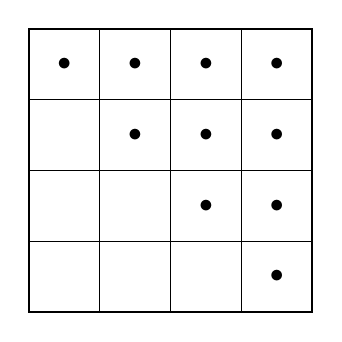
\begin{tikzpicture}[scale=0.9]
\draw[thick] (0,0) rectangle (4,4);
\foreach \x in {1,2,3} {
  \draw (\x,0) -- (\x,4);
}
\foreach \y in {1,2,3} {
  \draw (0,\y) -- (4,\y);
}
\foreach \x/\y in {
  0.5/3.5, 1.5/3.5, 2.5/3.5, 3.5/3.5,
  1.5/2.5, 2.5/2.5, 3.5/2.5,
  2.5/1.5, 3.5/1.5,
  3.5/0.5
} {
  \node at (\x,\y) {$\bullet$};
}
\end{tikzpicture}
\caption{A schematic symmetric \(4\times 4\) tensor. The diagonal and one triangular half contain the ten independent components.}
\end{figure}

For an antisymmetric tensor, the diagonal must vanish, since \(T^{\mu\mu}=-T^{\mu\mu}\). The remaining independent entries occupy only one triangular half of the matrix, so there are
\begin{equation}
6
\end{equation}
independent components. That number is exactly what we need for the three components of \(\vec E\) and the three components of \(\vec B\).

This is the point at which the electromagnetic field tensor enters. The secure identifications in the lecture are
\begin{equation}
E_1=f_{10},\qquad E_2=f_{20},\qquad E_3=f_{30},
\end{equation}
together with the cyclic magnetic pattern
\begin{equation}
f_{12}=-B_3,\qquad f_{23}=-B_1,\qquad f_{31}=-B_2.
\end{equation}
In the lecture's \((1,2,3,0)\) ordering, the electric field sits in the space-time slots and the magnetic field sits in the space-space slots.

A cautious first-pass matrix consistent with the transcript is
\begin{equation}
f_{\mu\nu}\approx
\begin{pmatrix}
0 & -B_3 & B_2 & E_1\\
B_3 & 0 & -B_1 & E_2\\
-B_2 & B_1 & 0 & E_3\\
-E_1 & -E_2 & -E_3 & 0
\end{pmatrix},
\end{equation}
with the understanding that the exact sign convention should be checked once more against the full board before the final pass. What is not in doubt is the structure: \(f_{\mu\nu}\) is antisymmetric, it has six independent components, the purely spatial block carries the magnetic field, and the slots involving the time index carry the electric field.

There is also a distinctly three-dimensional point at the end of the lecture. The magnetic field has two identities. In four-dimensional spacetime it is part of the two-index antisymmetric tensor \(f_{\mu\nu}\). But if we ignore time and look only at the \(3\times 3\) spatial antisymmetric block, that block has three independent components, and those three components can be re-read as an ordinary spatial vector \(\vec B\). That identification is special to three spatial dimensions.

Susskind ends with a historical remark that is worth keeping in view. Einstein did not originally write special relativity in polished four-vector notation. Much of that packaging is Minkowski's contribution. But the conceptual drive was already there: the laws of nature ought to take a form that is the same in every reference frame.

\section{Summary}

The lecture begins with a fake law and uses it to force the real principle onto the stage: the laws of physics must be written in forms that survive changes of coordinates. First we see this under rotations, then under Lorentz transformations. That is why collision laws are written as statements about whole vectors vanishing or being equal, why four-vectors are defined by their transformation law, and why scalars are built by contracting one upstairs index with one downstairs index.

Once that language is in place, proper velocity and four-momentum become natural. The old Lorentz force law then reveals its weakness: electric and magnetic fields cannot be invariantly separated. The lecture therefore ends at the threshold of the next step, with the electromagnetic field assembled into the antisymmetric tensor \(f_{\mu\nu}\). The relativistic force law itself belongs to the continuation.